% questions.tex —— 2015 年·广东卷·文科 · 题目内容片段（无答案）
% 由 tools/generate_projects.py 依来源总账自 2015/2015_数学真题_广东文_试题.md 生成，勿手改（改源 MD 后重跑）


\gkpart{数学}

\begin{gktip}
\textbf{来源说明}：本题面依据固定源 PDF 全 2 页逐题核对（p1＝页 949：栏 1 标题与「一、选择题」1–10；栏 2「二、填空题」11–15（含第 15 题圆与切线几何图）与「三、解答题」节头、第 16 题；栏 3 第 17 题（频率分布直方图）及三小问；p2＝页 950：栏 1 第 18 题（三角形 PDC 与长方形 ABCD 的立体图）与第 19 题；栏 2 第 20 题；栏 3 第 21 题）。原卷为 \textbf{A3 横向三栏书刊合排}，阅读序＝左→中→右；\textbf{页脚仅印合订本书页页码 949／950}，\textbf{无页眉}；标题在栏 1 内排印。\textbf{全卷不印分值、不印题量}——三个节头逐字仅「一、选择题」「二、填空题」「三、解答题」；\textbf{源内未印「必做/选做」分节标注}（栏 2 顶部与第 13/14 题交界经 600 dpi 复核确认）；总分 150 为结构推断，\textbf{卷面无凭据}，本文件不作补写。

\textbf{源制作体系判定}（实测）：源\textbf{不是扫描件，而是 LaTeX（Computer Modern 系）重排产物}——\texttt{pdfimages -list} 零命中（全页无位图）；嵌入字体含中文 \textbf{STSong／STHeiti}，拉丁与数学 \textbf{LMRoman 系与 CM 系（CMR10／CMR7／CMMI10／CMMI7／CMSY10／CMSY7／CMEX10／MSAM10）}，另有 \textbf{TeX-vect10}（向量长箭头）；\textbf{无 CMMIB10}；文本层整体可读；根号上横线、分式横线、作答横线与全部箭头为矢量路径（\textbf{第 5 题选项 (D) 的根号、第 18 题 (1) 的「$\parallel$」为文本层丢失符号}，以像素为准）。

\textbf{标点与字样约定（实测）}：① \textbf{题号与句末}源内为半角 \texttt{.}，按全库约定写作全角「．」；② \textbf{正文句读}源内为\textbf{半角 ASCII}（\texttt{,} \texttt{.}）与半角圆括号，一律归一为全角「，」「：」「；」「？」「（）」（顿号照源）；③ \textbf{选项标号}半角「(A)」照录；④ \textbf{作答空}：选择为「（　）」（源为半角括号＋约 1 em 空档），填空为统一横线（源为 31.5 pt 矢量线段，写作 \texttt{\gkblank{}}）；⑤ \textbf{分数}均为显示风格（真分式），排印一律 \(\dfrac{a}{b}\)；⑥ \textbf{不等号}按 MSAM10 实测排 \(\geqslant\)／\(\leqslant\)；⑦ \textbf{向量}：本卷\textbf{无 CMMIB10}——一律为 TeX-vect10 长箭头 \(\overrightarrow{AB}\)（字母本体为常规斜体，不加粗）；⑧ \textbf{正体}：\(\sin\)／\(\cos\)／\(\tan\)／\(\operatorname{card}\)（LMRoman10）、虚数单位 \(\mathrm{i}\)（直立）、自然数集 \(\mathbf{N}\)（粗正体，非黑板体）；⑨ 词间空格照页面词界补。

\textbf{存疑与登记}（源内异常一律照录；完整清单见工作档 \texttt{transcripts/partA.md}／\texttt{partB.md} 与 \texttt{figure-inventory.md}）：① \textbf{固定源不附参考答案}（等级 D）——解析全部由本库独立推导；② \textbf{第 5 题选项 (D) 的根号}为 CMSY10 根号字形＋独立矢量横线，文本层整枚丢失——按像素录 \(\sqrt{3}\)；③ \textbf{第 5 题「内角 \(A\)，\(B\)，\(C\) 的对边」中 C 后无逗号}（1200 dpi 复核确认真无）——照源不补；④ \textbf{第 18 题 (1) 的「$\parallel$」为矢量描边}（两笔斜线，文本层完全缺失；同题 (2) 的「\(\perp\)」为 CMSY10 字体字形，二者不同源）——按语义排印 \(\parallel\)；⑤ 第 18 题边 \(DC\) 自 \(D\) 起 13.6 pt 为\textbf{虚线段}（被棱 \(PA\) 遮挡的隐藏棱画法，虚线终点与 \(PA\cap DC\) 交点差 0.30 pt）——照源；⑥ 第 18 题图\textbf{未画棱 \(PB\)}——照源不补；⑦ 第 17 题断轴为\textbf{三齿 zigzag}（非「//」折断符），\(x\) 导引线与 \([240,260)\) 柱顶相差 0.117 pt——照源；⑧ 第 4 题约束条件三行以 cases 承托（源内「则…」与第二行同高，行列位置不复刻）；⑨ 答题空「( )」源内间距约 1.75 em，本库统一作「（　）」。
\end{gktip}

\gkpart{试题}

\gkpart{一、选择题}

\begin{question}
\gkti{1}若集合 \(M=\{-1,1\}\)，\(N=\{-2,1,0\}\)，则 \(M\cap N=\)（　）

(A) \(\{0,-1\}\)　(B) \(\{1\}\)　(C) \(\{0\}\)　(D) \(\{-1,1\}\)

\end{question}
\begin{question}
\gkti{2}已知 \(\mathrm{i}\) 是虚数单位，则复数 \((1+\mathrm{i})^2=\)（　）

(A) \(2\mathrm{i}\)　(B) \(-2\mathrm{i}\)　(C) \(2\)　(D) \(-2\)

\end{question}
\begin{question}
\gkti{3}下列函数中，既不是奇函数，也不是偶函数的是（　）

(A) \(y=x+\sin 2x\)　(B) \(y=x^2-\cos x\)

(C) \(y=2^x+\dfrac{1}{2^x}\)　(D) \(y=x^2+\sin x\)

\end{question}
\begin{question}
\gkti{4}若变量 \(x\)，\(y\) 满足约束条件

\nopagebreak[4]
\[
\begin{cases}
x+2y\leqslant 2,\\
x+y\geqslant 0,\\
x\leqslant 4,
\end{cases}
\]

则 \(z=2x+3y\) 的最大值为（　）

(A) \(2\)　(B) \(5\)　(C) \(8\)　(D) \(10\)

\end{question}
\begin{question}
\gkti{5}设 \(\triangle ABC\) 的内角 \(A\)，\(B\)，\(C\) 的对边分别为 \(a\)，\(b\)，\(c\)．若 \(a=2\)，\(c=2\sqrt{3}\)，\(\cos A=\dfrac{\sqrt{3}}{2}\) 且 \(b<c\)，则 \(b=\)（　）

(A) \(3\)　(B) \(2\sqrt{2}\)　(C) \(2\)　(D) \(\sqrt{3}\)

\end{question}
\begin{question}
\gkti{6}若直线 \(l_1\) 和 \(l_2\) 是异面直线，\(l_1\) 在平面 \(\alpha\) 内，\(l_2\) 在平面 \(\beta\) 内，\(l\) 是平面 \(\alpha\) 与平面 \(\beta\) 的交线，则下列命题正确的是（　）

(A) \(l\) 与 \(l_1\)，\(l_2\) 都不相交　(B) \(l\) 与 \(l_1\)，\(l_2\) 都相交

(C) \(l\) 至多与 \(l_1\)，\(l_2\) 中的一条相交　(D) \(l\) 至少与 \(l_1\)，\(l_2\) 中的一条相交

\end{question}
\begin{question}
\gkti{7}已知 \(5\) 件产品中有 \(2\) 件次品，其余为合格品，现从 \(5\) 件产品中任取 \(2\) 件，恰有一件次品的概率为（　）

(A) \(0.4\)　(B) \(0.6\)　(C) \(0.8\)　(D) \(1\)

\end{question}
\begin{question}
\gkti{8}已知椭圆 \(\dfrac{x^2}{25}+\dfrac{y^2}{m^2}=1\)（\(m>0\)）的左焦点为 \(F_1(-4,0)\)，则 \(m=\)（　）

\par\vspace*{3pt}

(A) \(2\)　(B) \(3\)　(C) \(4\)　(D) \(9\)

\end{question}
\begin{question}
\gkti{9}在平面直角坐标系 \(xOy\) 中，已知四边形 \(ABCD\) 是平行四边形，\(\overrightarrow{AB}=(1,-2)\)，\(\overrightarrow{AD}=(2,1)\)，则 \(\overrightarrow{AD}\cdot\overrightarrow{AC}=\)（　）

(A) \(5\)　(B) \(4\)　(C) \(3\)　(D) \(2\)

\end{question}
\begin{question}
\gkti{10}若集合 \(E=\{(p,q,r,s)\mid 0\leqslant p<s\leqslant 4,\ 0\leqslant q<s\leqslant 4,\ 0\leqslant r<s\leqslant 4\) 且 \(p,q,r,s\in\mathbf{N}\}\)，\(F=\{(t,u,v,w)\mid 0\leqslant t<u\leqslant 4,\ 0\leqslant v<w\leqslant 4\) 且 \(t,u,v,w\in\mathbf{N}\}\)，用 \(\operatorname{card}\,(X)\) 表示集合 \(X\) 中元素个数，则 \(\operatorname{card}\,(E)+\operatorname{card}\,(F)=\)（　）

(A) \(200\)　(B) \(150\)　(C) \(100\)　(D) \(50\)

\end{question}
\gkpart{二、填空题}

\begin{question}
\gkti{11}不等式 \(-x^2-3x+4>0\) 的解集为\gkblank{}．（用区间表示）

\end{question}
\begin{question}
\gkti{12}已知样本数据 \(x_1\)，\(x_2\)，\(\cdots\)，\(x_n\) 的均值 \(\bar{x}=5\)，则样本数据 \(2x_1+1\)，\(2x_2+1\)，\(\cdots\)，\(2x_n+1\) 的均值为\gkblank{}．

\end{question}
\begin{question}
\gkti{13}若三个正数 \(a\)，\(b\)，\(c\) 成等比数列，其中 \(a=5+2\sqrt{6}\)，\(c=5-2\sqrt{6}\)，则 \(b=\)\gkblank{}．

\end{question}
\begin{question}
\gkti{14}在平面直角坐标系 \(xOy\) 中，以原点 \(O\) 为极点，\(x\) 轴的正半轴为极轴建立极坐标系，曲线 \(C_1\) 的极坐标方程为 \(\rho(\cos\theta+\sin\theta)=-2\)，曲线 \(C_2\) 的参数方程为 \(\begin{cases}x=t^2,\\ y=2\sqrt{2}\,t,\end{cases}\)（\(t\) 为参数），则 \(C_1\) 与 \(C_2\) 交点的直角坐标为\gkblank{}．

\Needspace{0.4\textheight}
\end{question}
\begin{question}
\gkti{15}如图，\(AB\) 为圆 \(O\) 的直径，\(E\) 为 \(AB\) 延长线上一点，过 \(E\) 作圆 \(O\) 的切线，切点为 \(C\)，过 \(A\) 作直线 \(EC\) 的垂线，垂足为 \(D\)．若 \(AB=4\)，\(CE=2\sqrt{3}\)，则 \(AD=\)\gkblank{}．
\nopagebreak[4]
\begin{center}% f2015gdw_q15_circle.tex — 2015 年高考数学·广东卷·文科 第 15 题（圆与切线）
%
% 【来源】`.work/phase3-b16/source/2015广东文.pdf`（SHA-256
%   0c27f1a08f837014066c636a3190b8fa7ad7e5a4494f204e60412293aea17e09），
%   第 1 页（合订本页 949）第 2 栏；内容对象 5。逐路径实测见
%   `.work/phase3-b16/figure-inventory.md` Q15 节。
%
% 【坐标口径】清单坐标为「真页 pt、原点左上、y 向下」。本图取
%   X0 = 526.4664（圆最左点 x），Y0 = 398.4110（圆最低点 y_top），
%   本地坐标  (x, y) = (x_page − X0, Y0 − y_top)，
%   即本地 x 向右、y 向上，1 单位 = 1 TeX pt；tikzpicture 用 x=1pt, y=1pt。
%   换算示例：圆心 (571.5954, 353.2830) → 本地 (45.1290, 45.1280)；
%   A (526.4672, 353.2830) → (0.0008, 45.1280)；E (661.8502, 353.2830) → (135.3838, 45.1280)。
%   清单中的真页坐标逐点写在每题注释里，便于反查。
%
% 【线宽/虚线】全部路径 line width = 0.398pt（源内容流 `0.398 w`）；无虚线。
%   圆为 4 段三次贝塞尔（不是 arc 算子）：控制点距端点 24.92pt，
%   κ = 24.92 / 45.125 = 0.55225，与标准 κ 一致（FI-S7）。
%
% 【照源复刻的存疑项】
%   FI-S6：切点 C = (594.16, 314.20) 不是折线顶点；DE 为整段直线，
%          标签 C 基线 (594.96, 312.86) 相对切点偏移 (+0.80, −1.34) pt，照录。
%   FI-S7：圆用 4 段三次贝塞尔路径级复现，不用 \draw circle 近似。
%   圆心点：源为 CMSY10 0x0F（`\bullet`）文本字形，文本矩阵含 0.6 缩放
%          （CMSY10 10.5pt × 0.6 = 6.3pt 有效），基线原点 (570.0200, 354.6828)；
%          此处用 node scale=0.6 复现同一缩放（实测 1200dpi 墨径 2.40pt，
%          与源 2.46pt 一致），非矢量圆点。不用 \fontsize{6.3pt}——那会
%          触发 CMSY6 光学字号替换，墨径偏大（2.82pt）。
%
% 【自验结果】见文件末尾。
%
% 元素计数：4 条路径（1 圆 = 4 段贝塞尔 + 3 直线段）、7 个标签
%   （A B C D E O + 圆心点）。
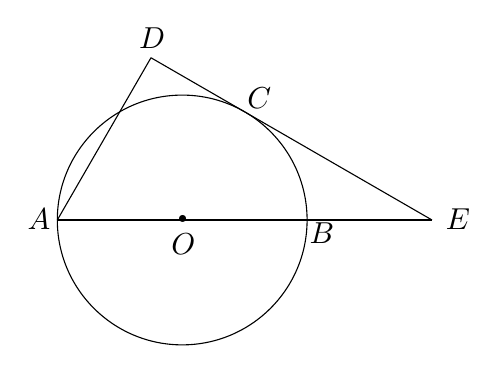
\begin{tikzpicture}[x=1pt, y=1pt,
    every node/.style={inner sep=0pt, font=\fontsize{10.5pt}{12.6pt}\selectfont}]

  % ---- 圆：m + 4c + h（源内容流 path 20，lw 0.398） ----
  % 源真页坐标：m (616.7234,353.2830)
  %   c (616.7234,328.3590) (596.5194,308.1550) (571.5954,308.1550)
  %   c (546.6714,308.1550) (526.4664,328.3590) (526.4664,353.2830)
  %   c (526.4664,378.2070) (546.6714,398.4110) (571.5954,398.4110)
  %   c (596.5194,398.4110) (616.7234,378.2070) (616.7234,353.2830)  h
  \draw[line width=0.398pt]
    (90.2570,45.1280)
    .. controls (90.2570,70.0520) and (70.0530,90.2560) .. (45.1290,90.2560)
    .. controls (20.2050,90.2560) and (0.0000,70.0520) .. (0.0000,45.1280)
    .. controls (0.0000,20.2040) and (20.2050,0.0000) .. (45.1290,0.0000)
    .. controls (70.0530,0.0000) and (90.2570,20.2040) .. (90.2570,45.1280)
    -- cycle;

  % ---- 垂线 AD（源 path 21，lw 0.398）：A(526.4672,353.2830) → D(560.3132,294.6600) ----
  \draw[line width=0.398pt] (0.0008,45.1280) -- (33.8468,103.7510);

  % ---- 直径延长线 AE（源 path 22，lw 0.398）：A(526.4672,353.2830) → E(661.8502,353.2830) ----
  \draw[line width=0.398pt] (0.0008,45.1280) -- (135.3838,45.1280);

  % ---- 切线 DE（源 path 23，lw 0.398）：D(560.3131,294.6605) → E(661.8501,353.2835) ----
  \draw[line width=0.398pt] (33.8467,103.7505) -- (135.3837,45.1275);

  % ---- 标签：源文本 Tm 原点（基线左端），CMMI10 10.5pt ----
  \node[anchor=base west] at (-10.9104,41.5400) {$A$};   % 源 (515.5560,356.8710)
  \node[anchor=base west] at (90.9416,36.6090)  {$B$};   % 源 (617.4080,361.8020)
  \node[anchor=base west] at (68.4956,85.5540)  {$C$};   % 源 (594.9620,312.8570)
  \node[anchor=base west] at (29.3546,107.1370) {$D$};   % 源 (555.8210,291.2740)
  \node[anchor=base west] at (140.1726,41.5400) {$E$};   % 源 (666.6390,356.8710)
  \node[anchor=base west] at (40.9786,32.5740)  {$O$};   % 源 (567.4450,365.8370)
  % 圆心点：源 CMSY10 0x0F（`\bullet`），Tm 为 0.6 缩放（CMSY10 10.5pt × 0.6），
  % 基线原点 (570.0200,354.6828) → 本地 (43.5536,43.7282)。
  \node[anchor=base west, scale=0.6] at (43.5536,43.7282) {$\bullet$};

\end{tikzpicture}
%
% 【自验结果】
%   探针：latexmk -pdfxe，0 error / 0 Overfull / 0 Underfull / 0 Missing character；
%         页面 162.34 × 114.08 pt（standalone border=0）。
%   tex 反算：4 条路径 + 7 个标签全部匹配，最大残差 0.000000 pt（阈值 0.05）。
%   600dpi 墨迹：整体墨迹包围盒最大边差 0.188 pt；几何包围盒 0.124 pt；
%         标签中心最大 0.240 pt（D）。（以上为尺度归一值，已扣除探针
%         0.996277 = 72/72.27 的 TeX pt / PDF bp 均匀因子）
%         按页面 bp 直接比较（物理）最大 0.604 pt，全部来自该 0.37% 均匀缩放。
%   灵敏度：端点 E +0.15pt → tex 检查器报 0.1500、600dpi 几何包围盒报 0.2409；
%         标签 C +0.15pt → tex 检查器报 0.1500、600dpi 标签中心报 0.1204。均能报出。
\end{center}
\nopagebreak[4]
\end{question}
\gkpart{三、解答题}

\begin{question}
\gkti{16}已知 \(\tan\alpha=2\)．

（1） 求 \(\tan\left(\alpha+\dfrac{\pi}{4}\right)\) 的值；

（2） 求 \(\dfrac{\sin 2\alpha}{\sin^2\alpha+\sin\alpha\cos\alpha-\cos 2\alpha-1}\) 的值．

\Needspace{0.4\textheight}
\end{question}
\begin{question}
\gkti{17}某城市 100 户居民的月平均用电量（单位：度），以 \([160,180)\)，\([180,200)\)，\([200,220)\)，\([220,240)\)，\([240,260)\)，\([260,280)\)，\([280,300)\) 分组的频率分布直方图如图．
\nopagebreak[4]
\begin{center}% f2015gdw_q17_histogram.tex — 2015 年高考数学·广东卷·文科 第 17 题（频率分布直方图）
%
% 【来源】`.work/phase3-b16/source/2015广东文.pdf`（SHA-256
%   0c27f1a08f837014066c636a3190b8fa7ad7e5a4494f204e60412293aea17e09），
%   第 1 页（合订本页 949）第 3 栏；内容对象 5。逐路径实测见
%   `.work/phase3-b16/figure-inventory.md` Q17 节。
%
% 【坐标口径】清单坐标为「真页 pt、原点左上、y 向下」。本图取
%   X0 = 862.9140（y 轴 x），Y0 = 345.5480（x 轴基线 y_top），
%   本地坐标  (x, y) = (x_page − X0, Y0 − y_top)，
%   即本地原点 = 坐标轴交点，x 向右、y 向上，1 单位 = 1 TeX pt。
%   换算示例：原点 (862.9140,345.5479) → (0, 0.0001)；
%   柱 [160,180) 左边界 (885.5915,345.5485) → (22.6775,−0.0005)；
%   y 轴箭头尖 (862.9140,127.1584) → (0,218.3896)。
%   y 轴箭头的旋转坐标系按 PDF 行向量右乘（后写 cm 先作用）换算（FI-S5）。
%
% 【线宽/虚线】轴线与柱体 line width = 0.398pt；分式横线 0.42pt；
%   两枚箭头为填充路径（源 `f`，无描边；源 lw=1.0，填充路径下线宽不参与着色），
%   包围盒 2.99 × 3.99pt；依赖 \usetikzlibrary{arrows.meta}（按库规加载；
%   箭头用路径级贝塞尔复刻，未用 Triangle 造型）；
%   虚线导引线 dash pattern = on 2.989pt off 2.989pt，dash phase = 0pt。
%
% 【照源复刻的存疑项】
%   FI-S4：x 导引线 y_top=228.6168，[240,260) 柱顶 y_top=228.5026，
%          相差 0.1142pt；照录（导引线与柱顶分别定位）。
%   FI-S5：y 轴箭头在 `0 1 -1 0 862.914 711.14509 cm` 旋转坐标系内，
%          按行向量右乘解析，箭头包围盒 x 861.42–864.41、y_top 127.16–131.14。
%   FI-S8：底部 0.0025 / 0.002 基线仅差 7.85pt，照录。
%   FI-S10：x 轴 160…300 八个刻度在源内为单个 TJ 以字距排开，
%          此处按逐点 Tm 起点分别定位（起点取自 pdftotext -bbox）。
%   断轴三齿折线逐点照录（11 点；振幅 ±2.339pt）。
%
% 【自验结果】见文件末尾。
%
% 元素计数：18 条路径（轴+断轴 1、箭头 2、分式线 1、柱 7、虚线导引 7）、
%   21 个文本标签。
\begin{tikzpicture}[x=1pt, y=1pt,
    every node/.style={inner sep=0pt, font=\fontsize{10.5pt}{12.6pt}\selectfont}]

  % ---- y 轴 + 断轴 + x 轴（源 path 26，14 点折线，lw 0.398） ----
  % 源真页坐标：m (862.9140,130.7449) l (862.9140,345.5479) l (867.4490,345.5479)
  %   l (868.5830,343.2099) l (870.8510,347.8869) l (871.9850,345.5479)
  %   l (873.1190,343.2099) l (875.3870,347.8869) l (876.5210,345.5489)
  %   l (877.6550,343.2099) l (879.9230,347.8869) l (881.0570,345.5489)
  %   l (885.5920,345.5489) l (1086.1030,345.5479)
  \draw[line width=0.398pt]
    (0.0000,214.8031) -- (0.0000,0.0001)
    -- (4.5350,0.0001) -- (5.6690,2.3381) -- (7.9370,-2.3389)
    -- (9.0710,0.0001) -- (10.2050,2.3381) -- (12.4730,-2.3389)
    -- (13.6070,-0.0009) -- (14.7410,2.3381) -- (17.0090,-2.3389)
    -- (18.1430,-0.0009) -- (22.6780,-0.0009) -- (223.1890,0.0001);

  % ---- y 轴箭头（源 path 27，两段贝塞尔，填充，无描边） ----
  % 源真页坐标（FI-S5 校正后）：尖 (862.9140,127.1584)
  %   c (862.7150,128.2214) (862.1170,129.9484) (861.4200,131.1434)
  %   l (864.4080,131.1434)
  %   c (863.7110,129.9484) (863.1130,128.2214) (862.9140,127.1584)
  \fill[line width=1.0pt]
    (0.0000,218.3896)
    .. controls (-0.1990,217.3266) and (-0.7970,215.5996) .. (-1.4940,214.4046)
    -- (1.4940,214.4046)
    .. controls (0.7970,215.5996) and (0.1990,217.3266) .. (0.0000,218.3896)
    -- cycle;

  % ---- x 轴箭头（源 path 28，两段贝塞尔，填充，无描边） ----
  % 源真页坐标：尖 (1089.6893,345.5480)
  %   c (1088.6263,345.3490) (1086.8993,344.7510) (1085.7043,344.0540)
  %   l (1085.7043,347.0420)
  %   c (1086.8993,346.3450) (1088.6263,345.7470) (1089.6893,345.5480)
  \fill[line width=1.0pt]
    (226.7753,0.0000)
    .. controls (225.7123,0.1990) and (223.9853,0.7970) .. (222.7903,1.4940)
    -- (222.7903,-1.4940)
    .. controls (223.9853,-0.7970) and (225.7123,-0.1990) .. (226.7753,0.0000)
    -- cycle;

  % ---- 「频率/组距」分式横线（源 path 29，lw 0.42） ----
  % 源真页坐标：(867.8080,127.8390) → (888.8080,127.8390)
  \draw[line width=0.42pt] (4.8940,217.7090) -- (25.8940,217.7090);

  % ---- 柱 [160,180)：源 path 30，m,l,l,l,h，lw 0.398 ----
  \draw[line width=0.398pt]
    (22.6775,31.1645) -- (22.6775,-0.0005) -- (45.3555,-0.0005)
    -- (45.3555,31.1645) -- cycle;
  % ---- 导引线 0.002：源 path 31，虚线 ----
  \draw[line width=0.398pt, dash pattern=on 2.989pt off 2.989pt, dash phase=0pt]
    (0.0000,31.1645) -- (22.6780,31.1645);

  % ---- 柱 [180,200)：源 path 32 ----
  \draw[line width=0.398pt]
    (45.3551,148.2099) -- (45.3551,-0.0001) -- (68.0331,-0.0001)
    -- (68.0331,148.2099) -- cycle;
  % ---- 导引线 0.0095：源 path 33 ----
  \draw[line width=0.398pt, dash pattern=on 2.989pt off 2.989pt, dash phase=0pt]
    (0.0000,148.2099) -- (45.3550,148.2099);

  % ---- 柱 [200,220)：源 path 34 ----
  \draw[line width=0.398pt]
    (68.0326,171.5239) -- (68.0326,-0.0001) -- (90.7106,-0.0001)
    -- (90.7106,171.5239) -- cycle;
  % ---- 导引线 0.011：源 path 35 ----
  \draw[line width=0.398pt, dash pattern=on 2.989pt off 2.989pt, dash phase=0pt]
    (0.0000,171.5239) -- (68.0330,171.5239);

  % ---- 柱 [220,240)：源 path 36 ----
  \draw[line width=0.398pt]
    (90.7101,194.8378) -- (90.7101,-0.0002) -- (113.3881,-0.0002)
    -- (113.3881,194.8378) -- cycle;
  % ---- 导引线 0.0125：源 path 37 ----
  \draw[line width=0.398pt, dash pattern=on 2.989pt off 2.989pt, dash phase=0pt]
    (0.0000,194.8378) -- (90.7100,194.8378);

  % ---- 柱 [240,260)：源 path 38（注意本柱顶无独立导引线，见 FI-S4） ----
  \draw[line width=0.398pt]
    (113.3877,117.0454) -- (113.3877,0.0004) -- (136.0657,0.0004)
    -- (136.0657,117.0454) -- cycle;

  % ---- 柱 [260,280)：源 path 39 ----
  \draw[line width=0.398pt]
    (136.0652,78.0303) -- (136.0652,0.0003) -- (158.7432,0.0003)
    -- (158.7432,78.0303) -- cycle;
  % ---- 导引线 0.005：源 path 40 ----
  \draw[line width=0.398pt, dash pattern=on 2.989pt off 2.989pt, dash phase=0pt]
    (0.0000,78.0303) -- (136.0650,78.0303);

  % ---- 柱 [280,300)：源 path 41 ----
  \draw[line width=0.398pt]
    (158.7427,39.0151) -- (158.7427,0.0001) -- (181.4207,0.0001)
    -- (181.4207,39.0151) -- cycle;
  % ---- 导引线 0.0025：源 path 42 ----
  \draw[line width=0.398pt, dash pattern=on 2.989pt off 2.989pt, dash phase=0pt]
    (0.0000,39.0151) -- (158.7430,39.0151);

  % ---- 导引线 x：源 path 43（y_top 228.6168，与柱顶差 0.1142pt，FI-S4） ----
  \draw[line width=0.398pt, dash pattern=on 2.989pt off 2.989pt, dash phase=0pt]
    (0.0000,116.9312) -- (113.3880,116.9312);

  % ---- 文本标签：源 Tm/Td 基线原点，10.5pt ----
  % 「频率/组距」：STSong；源基线 (867.8080,123.3610) / (867.8080,137.6670)
  \node[anchor=base west] at (4.8940,222.1870) {频率};
  \node[anchor=base west] at (4.8940,207.8810) {组距};
  % y 轴刻度值（源 C0_1 LMRoman10；基线左端）
  \node[anchor=base west] at (-32.8680,191.4570) {$0.0125$};  % 源 (830.0460,154.0910)
  \node[anchor=base west] at (-27.6180,168.1430) {$0.011$};   % 源 (835.2960,177.4050)
  \node[anchor=base west] at (-32.8680,144.8290) {$0.0095$};  % 源 (830.0460,200.7190)
  \node[anchor=base west] at (-9.7000,114.6710)  {$x$};       % 源 (853.2140,230.8770) CMMI10
  \node[anchor=base west] at (-27.6180,74.6490)  {$0.005$};   % 源 (835.2960,270.8990)
  \node[anchor=base west] at (-32.8680,35.6340)  {$0.0025$};  % 源 (830.0460,309.9140)
  \node[anchor=base west] at (-27.6180,27.7830)  {$0.002$};   % 源 (835.2960,317.7650)
  % 原点 0（源 (860.2890,356.2400)）
  \node[anchor=base west] at (-2.6250,-10.6920) {$0$};
  % x 轴刻度（源为单个 TJ；以下为逐点 Tm 起点，基线 y_top=356.0140）
  \node[anchor=base west] at (14.8020,-10.4660)  {$160$};  % 源 (877.716000,356.014)
  \node[anchor=base west] at (37.4800,-10.4660)  {$180$};  % 源 (900.394005,356.014)
  \node[anchor=base west] at (60.1570,-10.4660)  {$200$};  % 源 (923.071002,356.014)
  \node[anchor=base west] at (82.8350,-10.4660)  {$220$};  % 源 (945.749007,356.014)
  \node[anchor=base west] at (105.5130,-10.4660) {$240$};  % 源 (968.427012,356.014)
  \node[anchor=base west] at (128.1900,-10.4660) {$260$};  % 源 (991.104009,356.014)
  \node[anchor=base west] at (150.8680,-10.4660) {$280$};  % 源 (1013.782014,356.014)
  \node[anchor=base west] at (173.5450,-10.4660) {$300$};  % 源 (1036.459011,356.014)
  % x 轴标题「月平均用电量/度」：源三段分别定位，同一基线 (…,339.2240)
  \node[anchor=base west] at (187.4000,6.3240) {月平均用电量};  % 源 (1050.3140,339.2240) STSong
  \node[anchor=base west] at (250.4000,6.3240) {/};             % 源 (1113.3140,339.2240) LMRoman10
  \node[anchor=base west] at (255.6500,6.3240) {度};            % 源 (1118.5640,339.2240) STSong

\end{tikzpicture}
%
% 【自验结果】
%   探针：latexmk -pdfxe，0 error / 0 Overfull / 0 Underfull / 0 Missing character；
%         页面 301.40 × 240.11 pt（standalone border=0）。
%   tex 反算：18 条路径 + 21 个标签全部匹配，最大残差 0.000020 pt（阈值 0.05）。
%   600dpi 墨迹：整体墨迹包围盒最大边差 0.278 pt；几何包围盒 0.213 pt；
%         标签中心最大 0.273 pt（280）。（尺度归一，已扣除 0.996277 的
%         TeX pt / PDF bp 均匀因子）
%         按页面 bp 直接比较（物理）最大 0.952 pt（几何包围盒），来自该 0.37% 均匀缩放。
%   灵敏度：y 轴线宽 +0.02pt → 600dpi 等效线宽 +0.0358（tex 检查器不检线宽，报 0）；
%         刻度 200 y +0.15pt → tex 检查器报 0.1500、600dpi 标签中心报 0.2409。均能报出。
\end{center}
\nopagebreak[4]
（1） 求直方图中 \(x\) 的值；

（2） 求月平均用电量的众数和中位数；

（3） 在月平均用电量为 \([220,240)\)，\([240,260)\)，\([260,280)\)，\([280,300)\) 的四组用户中，用分层抽样的方法抽取 11 户居民，则月平均用电量在 \([220,240)\) 的用户中应抽取多少户？

\Needspace{0.4\textheight}
\end{question}
\begin{question}
\gkti{18}如图，三角形 \(PDC\) 所在的平面与长方形 \(ABCD\) 所在的平面垂直，\(PD=PC=4\)，\(AB=6\)，\(BC=3\)．
\nopagebreak[4]
\begin{center}% f2015gdw_q18_solid.tex — 2015 年高考数学·广东卷·文科 第 18 题（四棱锥 P-ABCD 立体图）
%
% 【来源】`.work/phase3-b16/source/2015广东文.pdf`
%   （SHA-256 0c27f1a08f837014066c636a3190b8fa7ad7e5a4494f204e60412293aea17e09），
%   第 2 页（合订本页 950）第 1 栏；内容对象 20。逐路径实测见
%   `.work/phase3-b16/figure-inventory.md` Q18 节。
%
% 【坐标口径】清单坐标为「真页 pt、原点左上、y 向下」。本图取
%   X0 = 202.0221（顶点 A 的 x），Y0 = 274.11714（顶点 A 的 y_top），
%   本地坐标  (x, y) = (x_page − X0, Y0 − y_top)，
%   即本地原点 = 顶点 A，x 向右、y 向上，1 单位 = 1 TeX pt。
%   换算示例：A (202.0221,274.1171) → (0,0)；B (365.2908,274.1171) → (163.2687,0)；
%   C (389.7813,233.3000) → (187.7592,40.8171)；D (226.5127,233.3000) → (24.4906,40.8171)；
%   P (308.1470,161.3053) → (106.1249,112.8119)。
%
% 【线宽/虚线】全部棱 line width = 0.3985pt（源先写 0.59776 w 随即被 0.3985 w 覆盖）；
%   DC 短段 dash pattern = on 2.98883pt off 2.98883pt，dash phase = 0pt；
%   无填充、无 c 算子（全为 m/l 直线）。
%
% 【照源复刻的存疑项】
%   FI-S1：DC 自 D 起为虚线，虚线终点 x=240.1184（∩ PA 计算值 x≈240.42，
%          差 0.30pt）；虚线路径方向照源为「交点 → D」，相位 0 起于交点。
%   FI-S2：源未画棱 PB，照录不补。
%   FI-S3：源每条棱路径起点有零长度重复 moveto（共 8 处），按规范不复刻。
%   FI-S9：Q18(1) 的「∥」在正文行内（y_top 89.20–98.25），不属于图形区，
%          不在本图内绘制。
%
% 【自验结果】见文件末尾。
%
% 元素计数：8 条棱（PA / PC / PD / DA / AB / BC / DC 实线 + DC 虚线）、5 个标签。
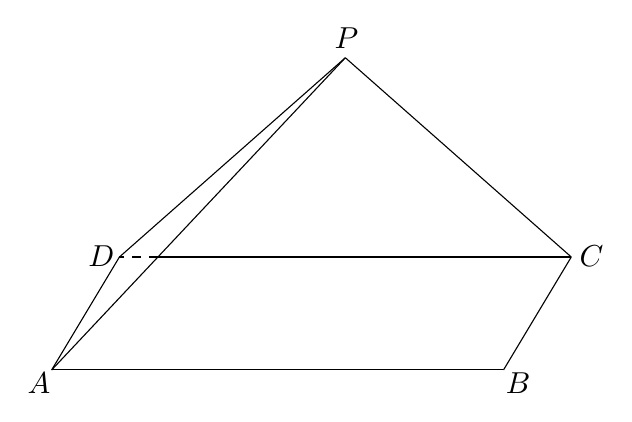
\begin{tikzpicture}[x=1pt, y=1pt,
    every node/.style={inner sep=0pt, font=\fontsize{10.5pt}{12.6pt}\selectfont}]

  % ---- 顶点（本地坐标） ----
  % A (0,0)  B (163.2687,0)  C (187.7592,40.8171)  D (24.4906,40.8171)  P (106.1249,112.8119)

  % ---- P–A（源 path 11：m A(202.0221,274.1171) l P(308.1470,161.3053)，本图反向） ----
  \draw[line width=0.3985pt] (106.1249,112.8119) -- (0.0000,0.0000);

  % ---- P–C（源 m (308.1470,161.3053) l (389.7813,233.3000)） ----
  \draw[line width=0.3985pt] (106.1249,112.8119) -- (187.7592,40.8171);

  % ---- P–D（源 path 3：m D(226.5127,233.3000) l P(308.1470,161.3053)，本图反向） ----
  \draw[line width=0.3985pt] (106.1249,112.8119) -- (24.4906,40.8171);

  % ---- D–A（源 path 7：m A(202.0221,274.1171) l D(226.5127,233.3000)，本图反向） ----
  \draw[line width=0.3985pt] (24.4906,40.8171) -- (0.0000,0.0000);

  % ---- A–B（源 path 9：m B(365.2908,274.1171) l A(202.0221,274.1171)，本图反向） ----
  \draw[line width=0.3985pt] (0.0000,0.0000) -- (163.2687,0.0000);

  % ---- B–C（源 m (365.2908,274.1171) l (389.7813,233.3000)） ----
  \draw[line width=0.3985pt] (163.2687,0.0000) -- (187.7592,40.8171);

  % ---- D–C 实线段（源 m (389.7813,233.3000) l (240.1184,233.3000)） ----
  \draw[line width=0.3985pt] (187.7592,40.8171) -- (38.0963,40.8171);

  % ---- D–C 虚线段（源 m (240.1184,233.3000) l (226.5127,233.3000)，方向照源） ----
  \draw[line width=0.3985pt, dash pattern=on 2.98883pt off 2.98883pt, dash phase=0pt]
    (38.0963,40.8171) -- (24.4906,40.8171);

  % ---- 标签：源文本 Tm 原点（基线左端），CMMI10 10.5pt ----
  \node[anchor=base west] at (102.0249,116.1981) {$P$};  % 源 (304.0470,157.9190)
  \node[anchor=base west] at (13.0239,37.2291)   {$D$};  % 源 (215.0460,236.8880)
  \node[anchor=base west] at (190.6049,37.2291)  {$C$};  % 源 (392.6270,236.8880)
  \node[anchor=base west] at (-8.8691,-8.5189)   {$A$};  % 源 (193.1530,282.6360)
  \node[anchor=base west] at (163.9539,-8.5189)  {$B$};  % 源 (365.9760,282.6360)

\end{tikzpicture}
%
% 【自验结果】
%   探针：latexmk -pdfxe，0 error / 0 Overfull / 0 Underfull / 0 Missing character；
%         页面 210.45 × 131.40 pt（standalone border=0）。
%   tex 反算：8 条棱 + 5 个标签全部匹配，最大残差 0.000057 pt（阈值 0.05）。
%   600dpi 墨迹：整体墨迹包围盒最大边差 0.285 pt；几何包围盒 0.064 pt；
%         标签中心最大 0.255 pt（C）。（尺度归一，已扣除 0.996277 的
%         TeX pt / PDF bp 均匀因子）
%         按页面 bp 直接比较（物理）最大 0.695 pt，来自该 0.37% 均匀缩放。
%   灵敏度：顶点 C x +0.15pt → tex 检查器报 0.1500、600dpi 几何包围盒报 0.1204。能报出。
\end{center}
\nopagebreak[4]
（1） 证明：\(BC\parallel\) 平面 \(PDA\)；

（2） 证明：\(BC\perp PD\)；

（3） 求点 \(C\) 到平面 \(PDA\) 的距离．

\end{question}
\begin{question}
\gkti{19}设数列 \(\{a_n\}\) 的前 \(n\) 项和为 \(S_n\)，\(n\in\mathbf{N}^{*}\)，已知 \(a_1=1\)，\(a_2=\dfrac{3}{2}\)，\(a_3=\dfrac{5}{4}\)，且当 \(n\geqslant 2\) 时，\(4S_{n+2}+5S_n=8S_{n+1}+S_{n-1}\)．

（1） 求 \(a_4\) 的值；

（2） 证明：\(\left\{a_{n+1}-\dfrac{1}{2}a_n\right\}\) 为等比数列；

（3） 求数列 \(\{a_n\}\) 的通项公式．

\end{question}
\begin{question}
\gkti{20}已知过原点的动直线 \(l\) 与圆 \(C_1: x^2+y^2-6x+5=0\) 相交于不同的两点 \(A\)，\(B\)．

（1） 求圆 \(C_1\) 的圆心坐标；

（2） 求线段 \(AB\) 的中点 \(M\) 的轨迹 \(C\) 的方程；

（3） 是否存在实数 \(k\)，使得直线 \(L: y=k(x-4)\) 与曲线 \(C\) 只有一个交点？若存在，求出 \(k\) 的取值范围；若不存在，说明理由．

\end{question}
\begin{question}
\gkti{21}设 \(a\) 为实数，函数 \(f(x)=(x-a)^2+|x-a|-a(a-1)\)．

（1） 若 \(f(0)\leqslant 1\)，求 \(a\) 的取值范围；

（2） 讨论 \(f(x)\) 的单调性；

（3） 当 \(a\geqslant 2\) 时，讨论 \(f(x)+\dfrac{4}{x}\) 在区间 \((0,+\infty)\) 内的零点个数．

\end{question}